% !TEX root = ../../../Lazcorreta.Tesis.tex

El preproceso es una de las fases que más tiempo consume en cualquier proceso de \KDD. No todos los valores registrados en el \texttt{Target Data} contienen información relevante para el estudio a realizar por lo que se deben eliminar todos aquellos que sólo aportan ruido o dificultan innecesariamente la ejecución de las siguientes fases del proceso.

Estas decisiones deben ser tomadas por expertos en la materia final del estudio, su experiencia puede agilizar enormemente el tiempo de obtención de resultados y la calidad de los mismos. La evaluación final puede ayudar también a tomar decisiones en esta fase si se detecta nula influencia de un dato incorporado en esta fase.

En el preproceso se decide qué hacer con los datos atípicos pues son datos que dificultan el estudio completo, decisión que aparecerá de nuevo en la fase de \dm. Pero su influencia puede ser esencial en algunas ocasiones. Hay investigadores que eliminan directamente estos datos atípicos, otros plantean un estudio exclusivo de estos datos. Sea cual sea la decisión tomada debería volverse a este punto una vez finalizado el proceso de \KDD para comprobar si puede explicarse de modo científico la existencia de datos atípicos (en ocasiones debidos simplemente a malas mediciones en el proceso de captación de datos).

También hay que tomar decisiones sobre los datos missing, incluso provocando un estudio previo para hacer una \prediccion sobre estos datos y poder utilizar estas estimaciones en el resto del proceso. Si un atributo posee muchos datos missing y se decide eliminar el atributo del estudio podríamos estar renunciando a información de extrema calidad, si se utilizan estimaciones de los mismos pero no son estimaciones correctas el resultado final puede aparecer totalmente sesgado por esta circunstancia.

\begin{wrapfigure}{o}{0.45\textwidth}
  \centering
  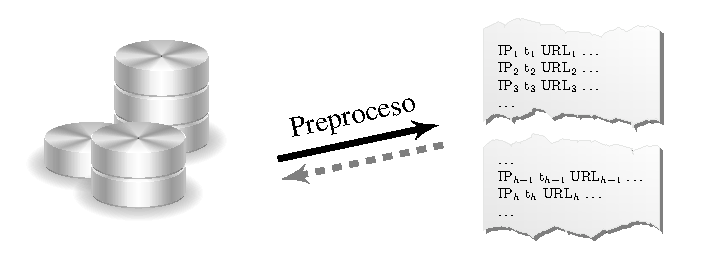
\includegraphics[width=.45\textwidth]{Preproceso.pdf}
	\caption{Preproceso}
	\label{fig:Preproceso}
\end{wrapfigure}
Al ser una de las fases que más recursos consume se llevará a cabo en horas en que el servidor tiene menor carga de trabajo y los resultados que ofrece serán usados posteriormente mediante algoritmos de extracción de información. Es fundamental crear los filtros adecuados al análisis posterior que se quiera realizar a estos datos, la extracción en sí de datos no es necesariamente compleja (puede ser una simple consulta a una \db) pero si no extraemos los datos adecuados la información obtenida puede carecer de relevancia.

Para estudiar el uso de un sitio web se deben conocer qué recursos ha solicitado realmente cada usuario. Considerando que una página web puede estar formada por gran cantidad de elementos: texto, imágenes, vídeos, anuncios externos o internos, enlaces\ldots es fácil pensar que cada vez que un usuario accede a un sitio web va a generar un gran número de líneas en su \flog, una por cada elemento incluido en la página solicitada y alojado en el servidor. La primera decisión a la hora de extraer información de los \flogs consiste en eliminar todas las líneas que no se deben a la navegación a través del sitio web por parte del usuario si no a la propia estructura del sitio web: se han de detectar las páginas que realmente ha solicitado el usuario y descartar los elementos que son cargados en el navegador del usuario por estar enlazados en la página solicitada~\citep{CooleyMobasherSrivastava-DataPreparationForMiningWWWBrowsingPatterns-1999}.

Además de eliminar toda esta información de los datos seleccionados en la fase previa hay muchas páginas solicitadas por los usuarios que realmente no existen en el servidor, marcadas con estado 404, que deben ser eliminadas después de analizar si se deben a una solicitud incorrecta escrita por el usuario o a enlaces propios del sitio web que han cambiado su ubicación o han desaparecido. Existen otros problemas en el uso de \flogs, como la existencia de páginas cargadas en la caché del servidor o del cliente y cuyas solicitudes no aparecerán~\citep{Pitkow-InSearchOfReliableUsageDataWWW-1997}. Algunos autores proponen resolverlo con el uso de "`huellas"'~\citep{VillenaGonzalezBarceloVelasco-MUWMedianteHuellasYSesiones-2002}. Otro problema es la existencia de agentes en la red (robots) que navegan automáticamente por todo un sitio web y cuyo comportamiento no debería ser considerado en el estudio ya que no reflejan el comportamiento de los usuarios a los que queremos adaptar el servicio.

Como en todos los procesos de \KDD, el preproceso reduce notablemente el número final de datos a analizar en \WUM. Sin embargo se debe vigilar que no se excluyan datos en esta fase que pudieran ser determinantes para la obtención de conocimiento de calidad.
